\documentclass{PDS}

\usepackage{graphicx}
\usepackage{caption}
\usepackage{subcaption}

\usepackage{amsmath}
\usepackage{amssymb}
\usepackage{amsfonts}
\usepackage{amsthm}

\usepackage[round]{natbib}

\usepackage{newtxtext}
\usepackage{newtxmath}

\usepackage{xcolor}
\usepackage[colorlinks,allcolors=dscolor,bookmarks=false]{hyperref}

\jyear{2025}
\jdoi{https://doi.org/10.1017/pds.2025.xxx}

\begin{document}

\title{First experiences from using CADdrive with digital LEGO for product design and systems engineering education}

\author{Georg Hackenberg}
\author{Christian Zehetner}

\address{School of Engineering, University of Applied Sciences Upper Austria, 4600 Wels, Austria}

\corresemail{georg.hackenberg@fh-wels.at}

\abstract{
Due to rising product and system complexities, design and engineering have become a team effort that requires well planned and synchronized activities to achieve high degrees of process efficiency and effectiveness.
In recent years, online collaboration platforms emerged which help managing all relevant project information in a central repository and, hence, speed up the information flow between the different stakeholders.
However, inspiring high school children to pursue a carreer in this field and preparing undergraduate as well as graduate students for what they will face in practice remains a challenge for institutions and societies worldwide.
To overcome the current situation, in this paper we present our experiences with conducting different course formats both with children from high school as well as with adults pursueing a Master-level study programme.
We provide insights into the organization of the different course formats, the various backgrounds and profiles of their participants, the work results produced by the individual teams, as well as the participants' feedback.
Overall, we conclude that online collaboration platforms like CADdrive with integrated version management, issue tracking, and task scheduling are well suited for conducting project-based courses with predefined design tasks.
In particular, our participants appreciated the transparency which can be achieved by means of online collaboration platforms as well as the accountability of the individual team members, which fosters active participation and learning.
}

\keywords{product design, systems engineering, engineering education}

\maketitle

\section{Introduction}
\label{sec:introduction}

With time, humanity is building ever more complex systems in different domains such as production, transportation, communication, and computation.
The growing complexity of these systems can be seen, for example, in the growing number of (atomic and composite) components, their interfaces, and their interactions.
Furthermore, the interfaces between these components typically are not limited to one engineering discipline (e.g.\ mechanics or electrics) anymore, but span several disciplines.
Ultimately, we deal with a mutlitude of mechatronic components providing required mechanical, electrical, and informational properties.

In the past, the ability to engineer such complex systems has been a major success factor for societies and organizations around the globe.
Today, due to rising competition in many domains the engineering ability alone is not sufficient anymore, but the efficiency and effectiveness of the underlying engineering processes must be taken into account.
In this context, \textit{efficiency} means that the overall engineering process can be executed as fast as possbile and the system's time-to-market is minimized.
In contrast, \textit{effectiveness} means that the engineering process consumes as little ressources as possible and, hence, unnecessary costs are avoided.

One key to efficiency is dividing the work into activities, which can be executed in parallel, but might require synchronization of their work results.
Furthermore, the individual activities must be scheduled such that the work results of one activity are ready when they are needed by another acitivity.
When required work results are not ready in time, you have two choices:
Either you delay follow-up activities potentially causing a suboptimal utilization of project resources such as personell and material.
Or you start follow-up activities anyways and risk working with wrong assumptions causing unnecessary future revisions of work results.

In contrast, one key to effectiveness is to understand stakeholder requirements and validate assumptions as early as possible in the engineering process.
Hence, validation activities must be planned where applicable to ensure that such mistakes are uncovered and resolved quickly and to minimize their impact on the future course of the project.
In this context, agile methodologies and frameworks have emerged over the past two decades ensuring stakeholder integration along the entire development process.
In the agile approach, stakeholders have the obligation to review work results frequently and give their feedback to the engineering team.

Today, online collaboration platforms with vision management, issue tracking, and task scheduling support engineering teams in achieving high degrees of efficiency and effectiveness.
The idea behind such platforms is to bundle all relevant project information in a central repository, to which all stakeholders have access from anywhere and anytime.
Consequently, the speed of information flow between the stakeholders can be improved significantly compared to traditional approaches.
Higher speeds of information flow, in turn, reduce the risk of project delays as well as incorrect assumptions and unnecessary revisions of work results.

As academic teachers we try to prepare young engineers as good as possible for what they will face in practice after entering the job market.
Ideally, our graduates quickly find their place in multi-disciplinary engineering teams and contribute reliably to the success of their assigned projects.
Hence, beyond the core technical skills they need a solid understanding of the overall engineering processes, the overarching efficiency and effectiveness objectives, as well as the employed collaboration principles.
Teaching such profound understanding of process, team, and collaboration dynamics still remains a challenge for engineering education.

\paragraph{Research question}

To overcome the current situation in engineering education, we wanted to understand how well different course formats and settings work based on a representative online collaboration platform, the digital LEGO framework, and classical CAD.
In particular, we wanted to understand the suitability of different course formats as well as the underlying platform and framework for Master-level product design and systems engineering education.
Furthermore, we were interested in how well such course formats work for children from high school aged between 10 and 15 years old, how well they can deal with CAD programs, and how well they understand collaboration challenges.

\paragraph{Contribution}

To answer the previous research questions, we conducted three Master-level courses on product design and systems engineering as well as one workshop with high school children.
The organizational structure of the three Master-level courses as well as the workshop, and the work results of the different teams are explained in Section~\ref{sec:contribution}.
During and after conducting the experiments we collected feedback from the individual participants and analyzed the data as discussed in Section~\ref{sec:discussion}.
Finally, we draw our conclusions from the previous experiments and their data, derive our key learnings, and sketch out important future work towards high impact engineering education in Section~\ref{sec:conclusion}.

\section{Course experiments}
\label{sec:contribution}

For our experiements we used the open source software CADdrive\footnote{\url{https://github.com/ghackenberg/caddrive}} as the underlying online collaboration platform with version management, issue tracking, and task scheduling, as well as the open source software LeoCAD\footnote{\url{https://github.com/leozide/leocad}} for digital LEGO design.
% and  Dassault Systèmes SolidWorks\footnote{\url{https://www.solidworks.com/}} for classical CAD.
Subsequently, we first describe our Master-level course formats with students at University of Applied Sciences Upper Austria in Section~\ref{sec:master}, before explaining our workshop format with high school children in Section~\ref{sec:school}.
Both for the Master-level courses and the workshop we introduce the organizational settings and show the most interesting work results delivered by the individual teams.

\subsection{Master level}
\label{sec:master}

At Master level, we conducted two different courses in two independent study programmes with slightly varied study plans and, hence, organizational settings.
The goal of the first course was to design a energy-optimal glasshouse for growing sweet tomatos over the winter months in Alpine regions as explained in Section~\ref{sec:master-product-lego}.
Furthermore, the course included a fair amount of simulation tasks for verification and validation.
The goal of the second course was to design a paper folding machine turning plain paper sheets into boxes as expained in Section~\ref{sec:master-system-lego}.
However, the course did not include simulation tasks, but verification and validation was achieved through manual reviews only.
%And the goal of the thrid course was to design two innovative, but not otherwise constrained products in the vertical farming space as explained in Section~\ref{sec:master-product-classical}.

\subsubsection{Glasshouse for Alpine regions}
\label{sec:master-product-lego}

The first course started in the winter term 2023 in the full-time Master programme "Innovation and Product Management".
The participants included 5 women and 5 men between 26 and 40 years old having between 1 and 16 years of work experience in different industries (e.g.\ automotive, retail, banking, etc.) and departments (e.g.\ product development, logistics, martketng and sales, etc.).
Furthermore, 8 students were holding a Bachelor degree and 2 students were holding a Master degree in some field.
Also, most students were already familiar with some CAD tool (e.g.\ PTC Creo, AutoDesk AutoCAD, Siemens NX, etc.) as well as simulation software (e.g.\ Abaqus, Matlab Simulink, Ansys, etc.).

In this project-based course, the goal of the group was to design an energy-efficient glasshouse for growing sweet tomatos over the winter months in Alpine regions.
The tasks included requirements analysis, modular architecture design, mechanical design, electrical design, and simulation-based verification of selected system properties.
Figure~\ref{fig:glasshouse} shows the mechanical design developed by the group with digital LEGO bricks and LeoCAD.
The mechanical design comprises a grow area for the plants with glass walls and windows as well as solar panels on the roof (see Figure~\ref{fig:glasshouse_2}), and a shed area for storing tools and batteries (see Figure~\ref{fig:glasshouse_3}).

\begin{figure}[htbp]
    \begin{subfigure}[b]{0.32\textwidth}
        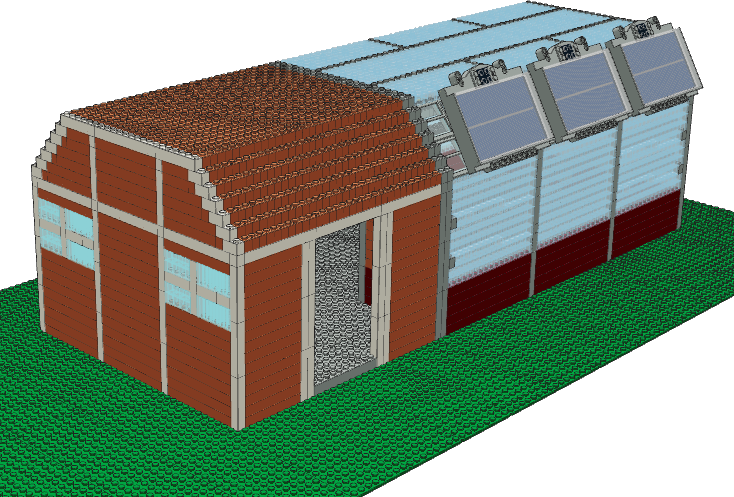
\includegraphics[width=\textwidth]{./figures/glasshouse_1.png}
        \caption{Exterior design}
        \label{fig:glasshouse_1}
    \end{subfigure}
    \hfill
    \begin{subfigure}[b]{0.32\textwidth}
        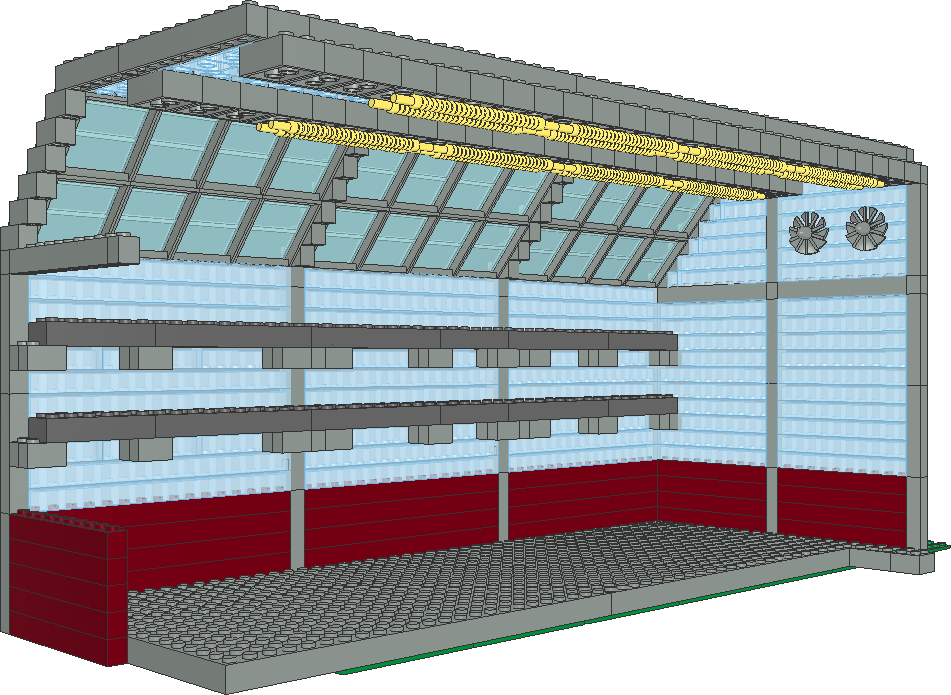
\includegraphics[width=\textwidth]{./figures/glasshouse_2.png}
        \caption{Interior design (grow area)}
        \label{fig:glasshouse_2}
    \end{subfigure}
    \hfill
    \begin{subfigure}[b]{0.32\textwidth}
        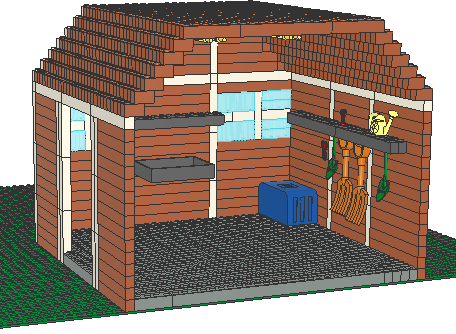
\includegraphics[width=\textwidth]{./figures/glasshouse_3.png}
        \caption{Interior design (shed area)}
        \label{fig:glasshouse_3}
    \end{subfigure}
    \caption{Mechanical design of the glasshouse with digital LEGO bricks.}
    \label{fig:glasshouse}
\end{figure}

In the context of simulation-based verification, the group was tasked with applying finite element analysis (FEA), computational fluid dynamics (CFD), and multi-physics simulation (MPS) for analyzing selected system properties.
The group decided to apply finite element analysis for analyzing the stability of the mechanical structure under snow and wind pressure, as well as computational fluid dynamics for analyzing the heat loss characteristics of the building.
Furthermore, the group decided to employ multi-physics simulation with OpenModelica\footnote{\url{https://github.com/OpenModelica/OpenModelica}} for analyzing the electrical energy consumption caused by the automatic window opening and closing system as shown in Figure~\ref{fig:glasshouse-sim}.

\begin{figure}[htbp]
    \begin{subfigure}[b]{0.575\textwidth}
        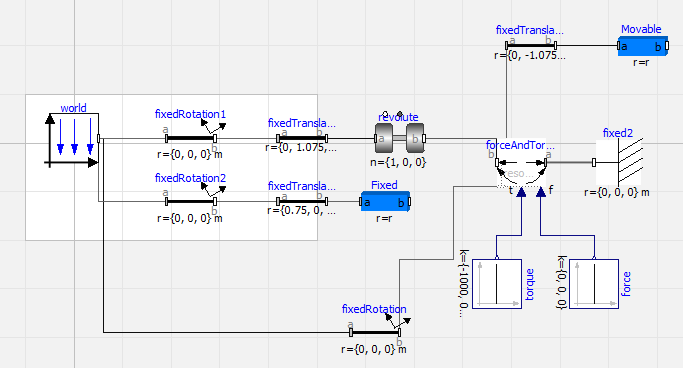
\includegraphics[width=\textwidth]{./figures/glasshouse_mechatronic_1.png}
        \caption{OpenModelica component model}
        \label{fig:glasshouse-sim-1}
    \end{subfigure}
    \hfill
    \begin{subfigure}[b]{0.41\textwidth}
        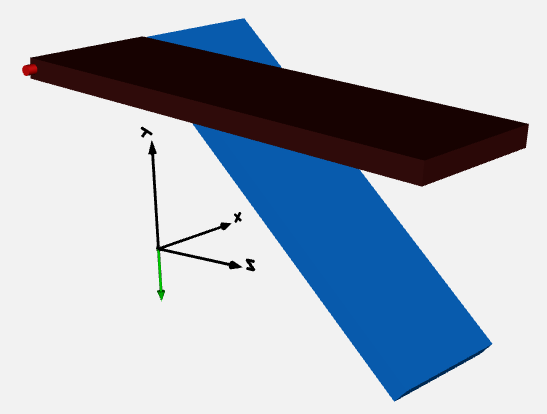
\includegraphics[width=\textwidth]{./figures/glasshouse_mechatronic_2.png}
        \caption{3D visualization}
        \label{fig:glasshouse-sim-2}
    \end{subfigure}
    \caption{Multi-physics simulation of automatic window opening and closing system.}
    \label{fig:glasshouse-sim}
\end{figure}

% TODO

\subsubsection{Paper folding machines}
\label{sec:master-system-lego}

The second course also started in the winter term 2023 in the part-time Master programme "Robotic Systems Engineering".
The participants included 1 woman and 12 men between 25 and 33 years old having between 3 and 10 years of work experience in different industries (e.g.\ logistics, chemical, agriculture, etc.) and departmets (e.g.\ automation engineering, business development, project management, etc.).
Furthermore, all students were holding a Bachelor degree in some technical field.
Also, most students were familar with some CAD software (e.g.\ AutoDesk AutoCAD, Dassault Systèmes Catia, PTC Creo, etc.), while only two students did not have prior CAD experience.

The course was divided into two parts, a theory part followed by a practice part.
In the theory part different concepts such as systems engineering, systems lifecycle processes, requirements analysis, systems architecture, systems integration, as well as verification and validation were introduced.
In the practice part the students were split into teams and were given the goal of developing a paper folding machine, which turns plain paper sheets into boxes with defined measures.
The tasks included requirements analysis, mechatronic systems architecture derivation, as well as mechanical, electrical, and logical system design.
Figure~\ref{fig:paper} shows three different mechanical designs proposed by the teams.

\begin{figure}[htbp]
    \begin{subfigure}[b]{0.32\textwidth}
        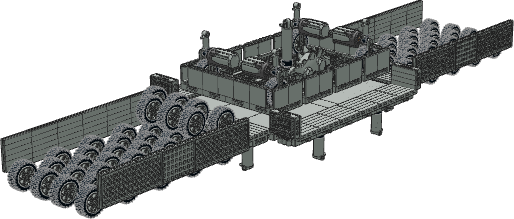
\includegraphics[width=\textwidth]{./figures/paper_1.png}
        \caption{First team}
        \label{fig:paper_1}
    \end{subfigure}
    \hfill
    \begin{subfigure}[b]{0.32\textwidth}
        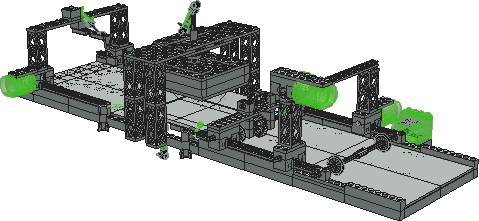
\includegraphics[width=\textwidth]{./figures/paper_2.png}
        \caption{Second team}
        \label{fig:paper_2}
    \end{subfigure}
    \hfill
    \begin{subfigure}[b]{0.32\textwidth}
        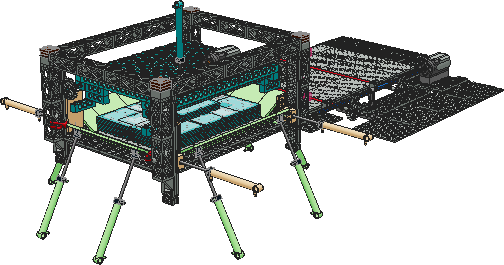
\includegraphics[width=\textwidth]{./figures/paper_3.png}
        \caption{Third team}
        \label{fig:paper_3}
    \end{subfigure}
    \caption{Different mechanical designs of the paper folding machine.}
    \label{fig:paper}
\end{figure}

In contrast, Figure~\ref{fig:paper-sub} shows the electrical and logical design of one paper folding machine.
This particular team worked with EPLAN Electric P8\footnote{\url{https://www.eplan-software.com/solutions/eplan-electric-p8/}} for the electrical design as well as Excalidraw\footnote{\url{https://excalidraw.com/}} for the logical design of the target system.
Note that in this case one student was already familiar with EPLAN Electric P8, which is why the first tool was selected.
Furhtermore, note that the notation for the logical design was not prescribed by the course instructor, but resembles some form of state chart formalism, which is common in control engineering.
Finally, validation of the different designs was performed with manual review techniques across all teams.

\begin{figure}[htbp]
    \centering
    \begin{subfigure}[b]{0.4\textwidth}
        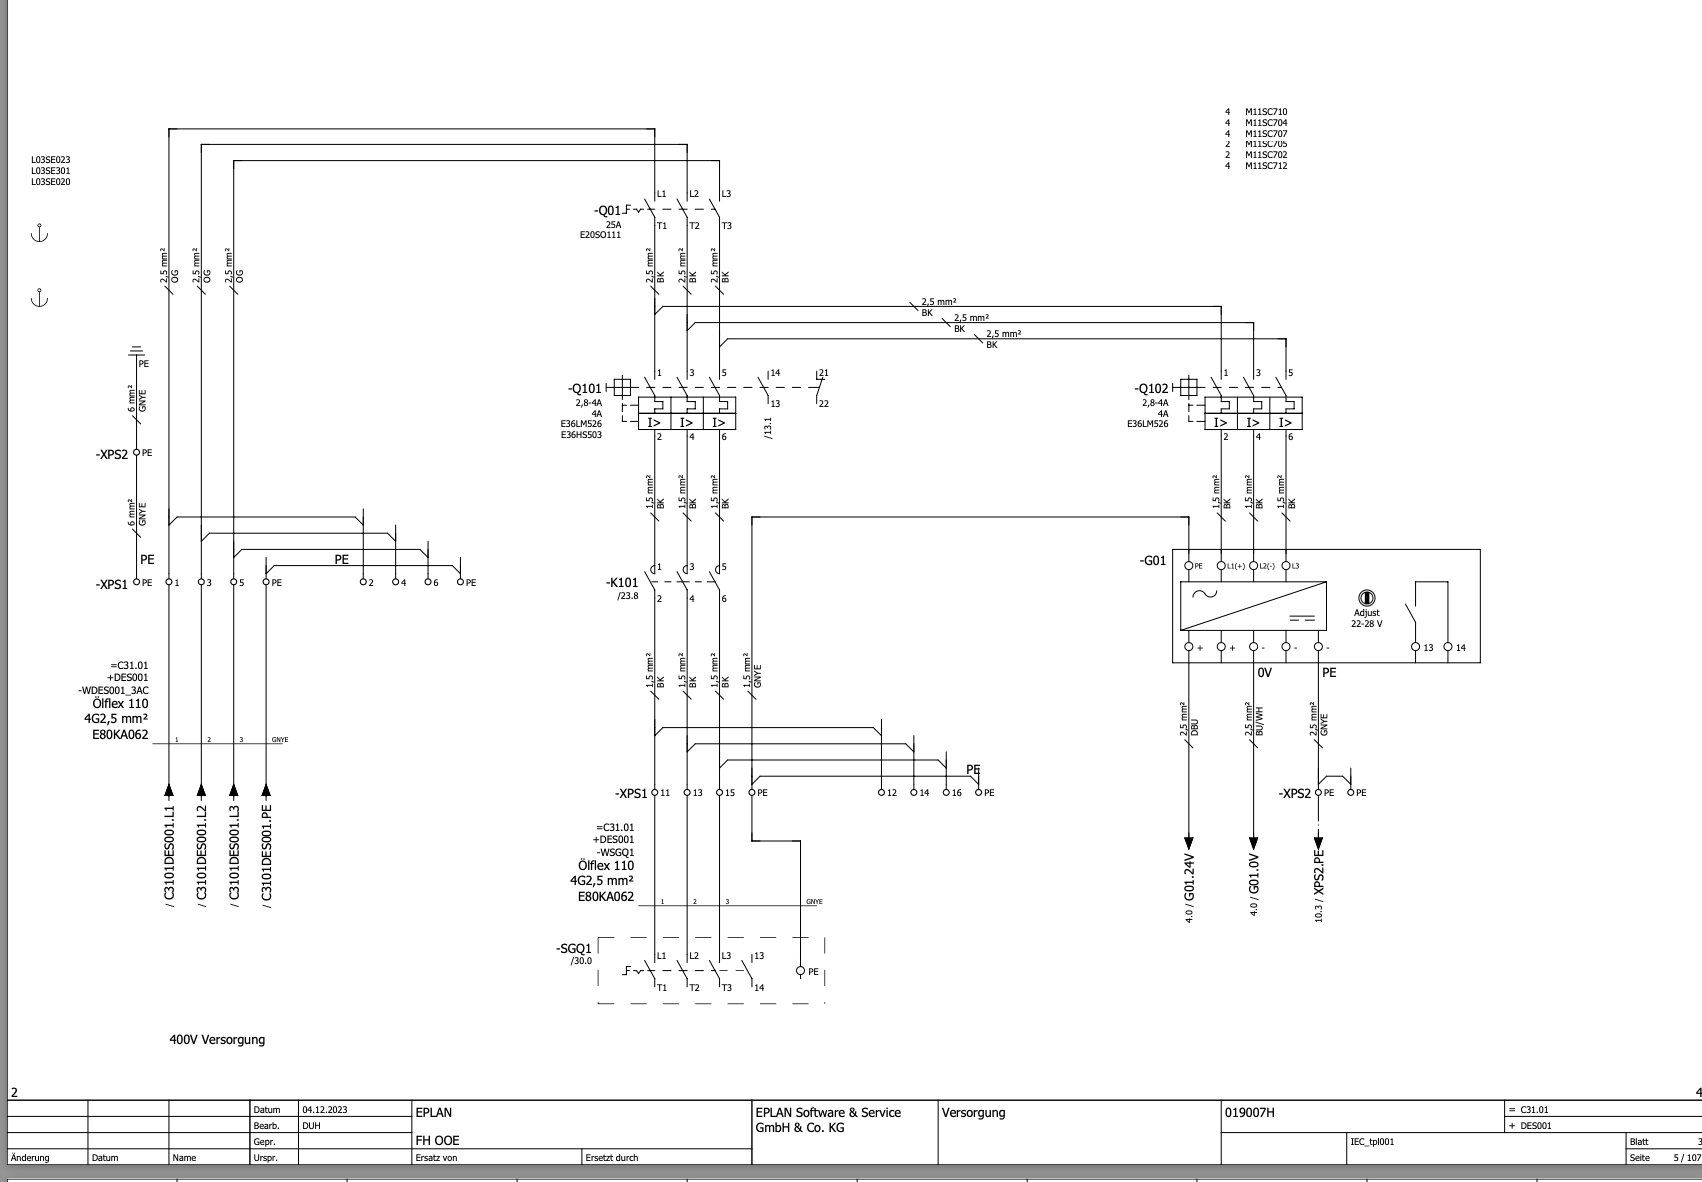
\includegraphics[width=\textwidth]{./figures/paper_electric.png}
        \caption{Electrical design}
        \label{fig:paper-sub-1}
    \end{subfigure}
    \hspace{0.05\textwidth}
    \begin{subfigure}[b]{0.45\textwidth}
        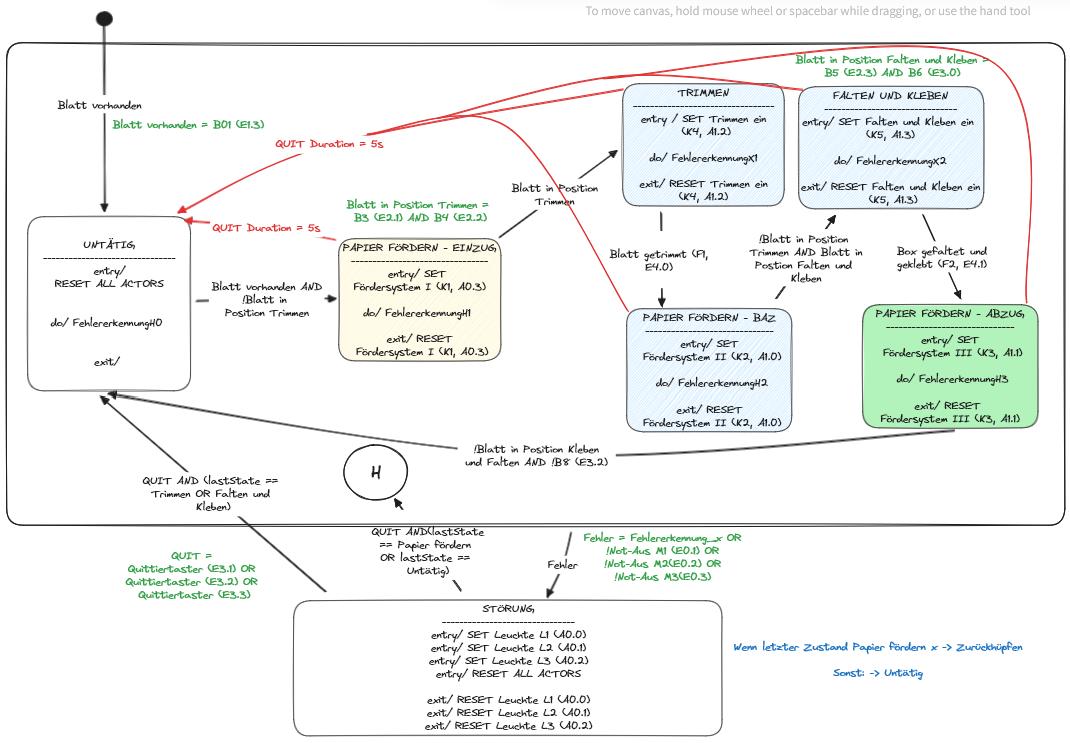
\includegraphics[width=\textwidth]{./figures/paper_control.png}
        \caption{Logical design}
        \label{fig:paper-sub-2}
    \end{subfigure}
    \caption{Electrical and logical design of one paper folding machine.}
    \label{fig:paper-sub}
\end{figure}

% TODO

% \subsubsection{Vertical farming products}
% \label{sec:master-product-classical}

% TODO

% \begin{figure}[htbp]
%     \begin{subfigure}[b]{0.27\textwidth}
%         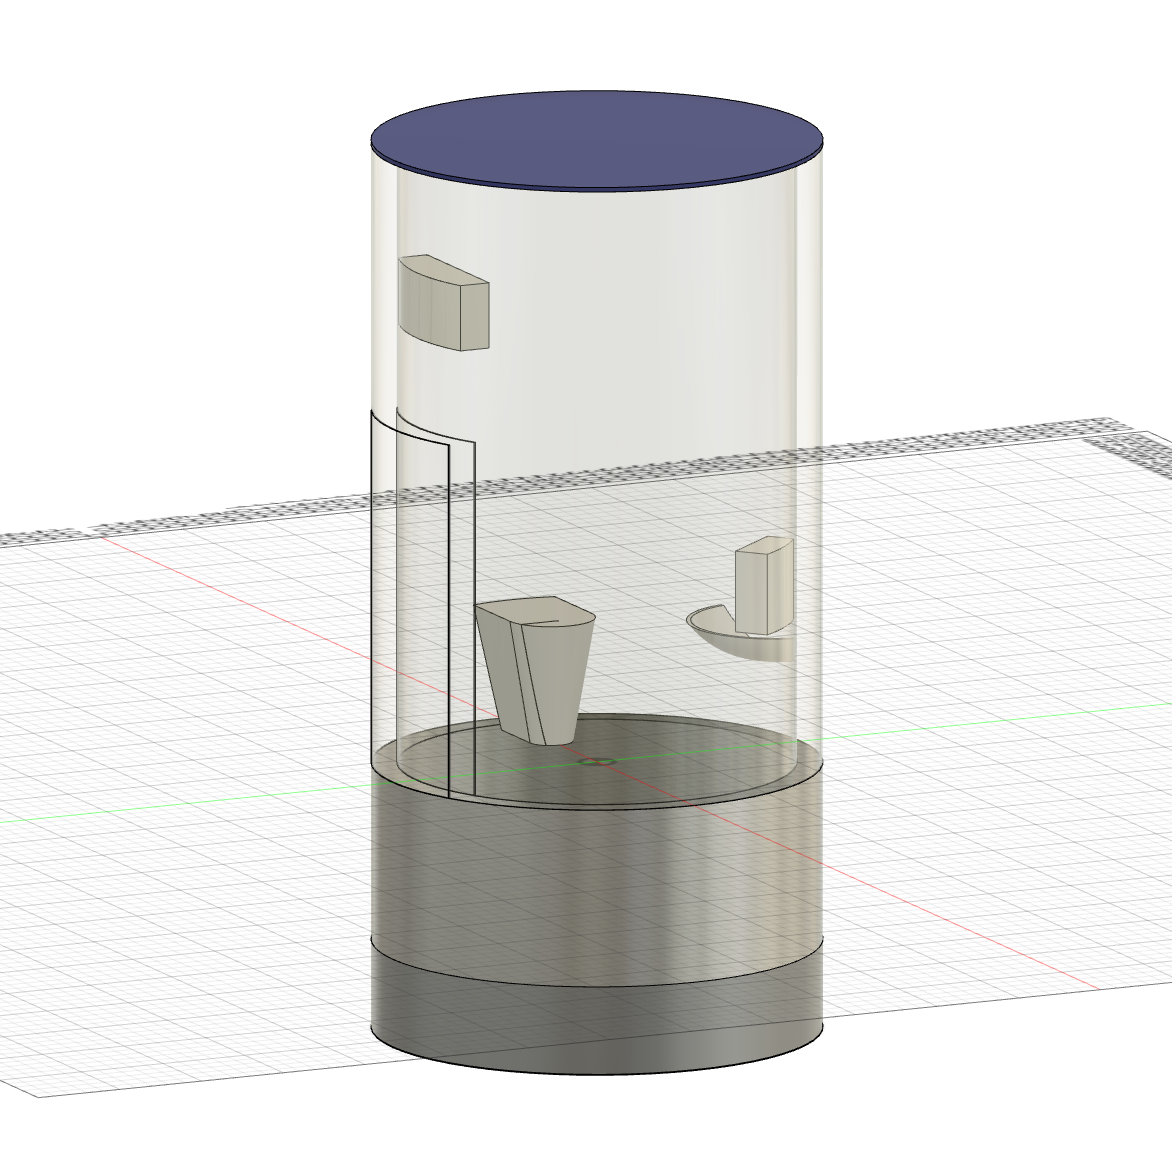
\includegraphics[width=\textwidth]{./figures/ecoflush.png}
%         \caption{EcoFlush}
%     \end{subfigure}
%     \hfill
%     \begin{subfigure}[b]{0.375\textwidth}
%         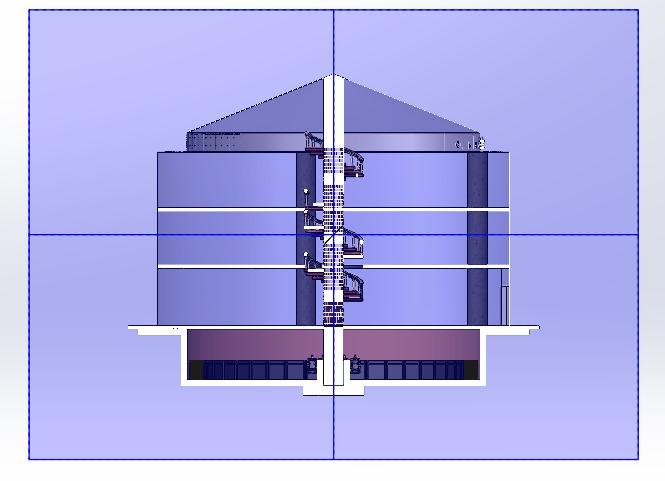
\includegraphics[width=\textwidth]{./figures/golazo-1.jpg}
%         \caption{Golazo building}
%     \end{subfigure}
%     \hfill
%     \begin{subfigure}[b]{0.27\textwidth}
%         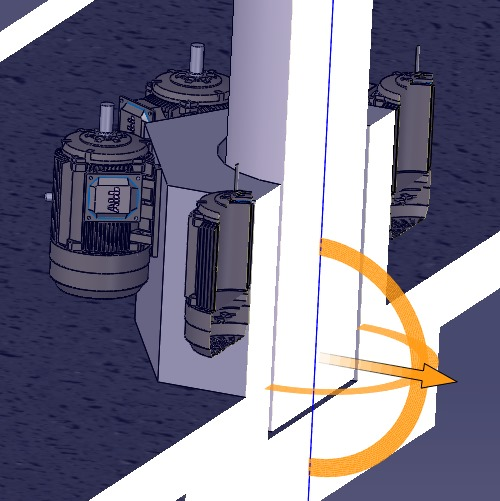
\includegraphics[width=\textwidth]{./figures/golazo-2.jpg}
%         \caption{Golazo engine}
%     \end{subfigure}
%     \caption{Mechanical designs.}
% \end{figure}

% TODO

% \begin{figure}
%     \begin{subfigure}[b]{0.49\textwidth}
%         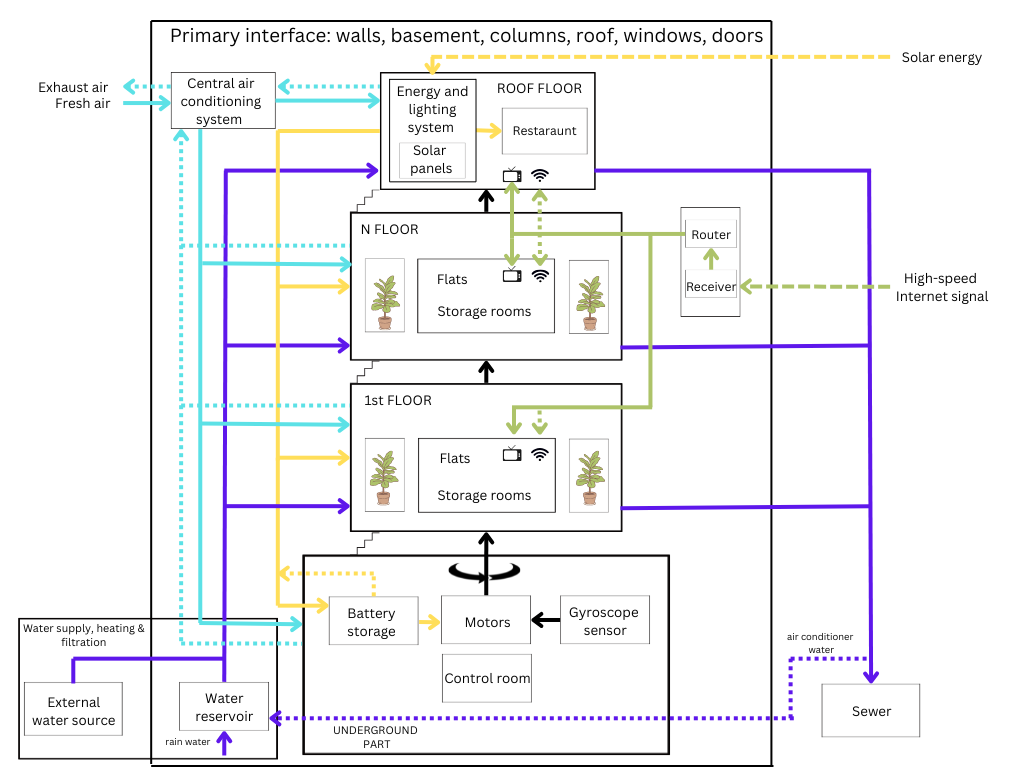
\includegraphics[width=\textwidth]{./figures/golazo-structure.png}
%         \caption{Module architecture}
%     \end{subfigure}
%     \hfill
%     \begin{subfigure}[b]{0.49\textwidth}
%         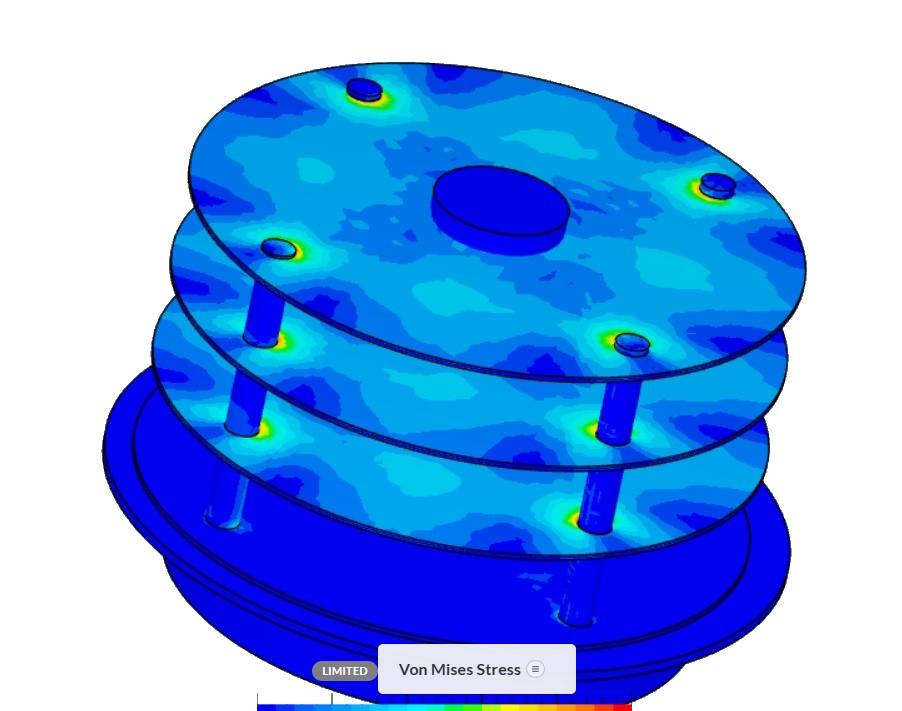
\includegraphics[width=\textwidth]{./figures/golazo-sim.jpg}
%         \caption{Static simulation}
%     \end{subfigure}
%     \caption{Module architecture and static simulation.}
% \end{figure}

% TODO

\subsection{High school level}
\label{sec:school}

At high school level, we conducted one single-day workshop with children from around Wels city in Upper Austria.
The workshop was organized as part of the KinderUni\footnote{\url{https://www.kinderuni-ooe.at/}} summer programme at the the School of Engineering of the University of Applied Sciences of Upper Austria in Wels, Austria.
The KinderUni programme provides children the chance to experience science hands-on and to learn about different topics such as engineering, biology, architecture, and many more.
Section~\ref{sec:school-lego} explains the structure of this single-day workshop and highlights results developed by the children during the course of the workshop.

\subsubsection{LEGO product ideas}
\label{sec:school-lego}

The workshop took place in July 2024 and was organized by the Upper Austrian branch of the KinderUni in Wels city\footnote{\url{https://www.kinderuni-ooe.at/kinderuni-ooe/wels/}}.
The workshop participants included 7 girls and 12 boys between 10 and 15 years old from different primary and high schools in the region, some -- but not all -- knowing each other from the same school.
In the morning, the children were brought to the School of Engineering of the University of Applied Sciences Upper Austria by their parents and were welcomed by an official representative of KinderUni.
The workshop itself lasted from morning until late afternoon and included short breaks before and after noon as well as a lunch break.

During the workshop, the hosts first presented the workshop agenda and the goal of the design projects before explaining and demonstrating the basics of LeoCAD for digital LEGO design.
Then the children were divided into teams of two with one girl working alone due to the uneven number of workshop participants.
The goal of each team was to develop an idea for a new LEGO product, while the target group (e.g.\ male or female), the target age (e.g.\ under 10, under 16, over 18, etc.), and the target theme (e.g.\ science fiction, princess, holiday, etc.) for the product could be selected freely.
Figure~\ref{fig:kinderuni} shows three product designs, which have been proposed by the teams.

\begin{figure}[htbp]
    \centering
    \begin{subfigure}[b]{0.21\textwidth}
        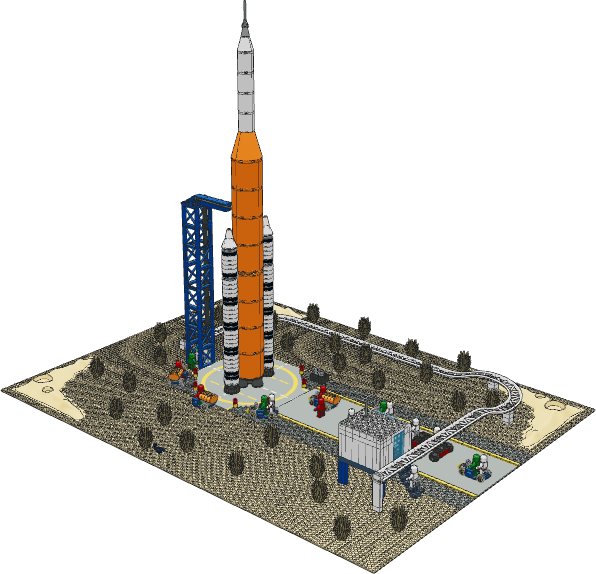
\includegraphics[width=\textwidth]{./figures/space.png}
        \caption{Space station}
        \label{fig:rocket}
    \end{subfigure}
    \hspace{0.05\textwidth}
    \begin{subfigure}[b]{0.21\textwidth}
        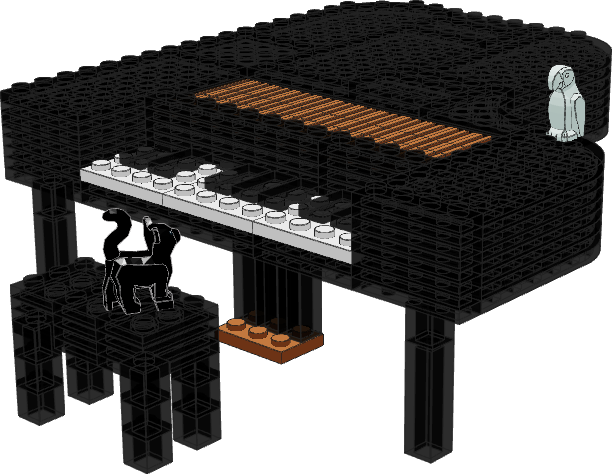
\includegraphics[width=\textwidth]{./figures/piano.png}
        \caption{Animal piano}
        \label{fig:piano}
    \end{subfigure}
    \hspace{0.05\textwidth}
    \begin{subfigure}[b]{0.21\textwidth}
        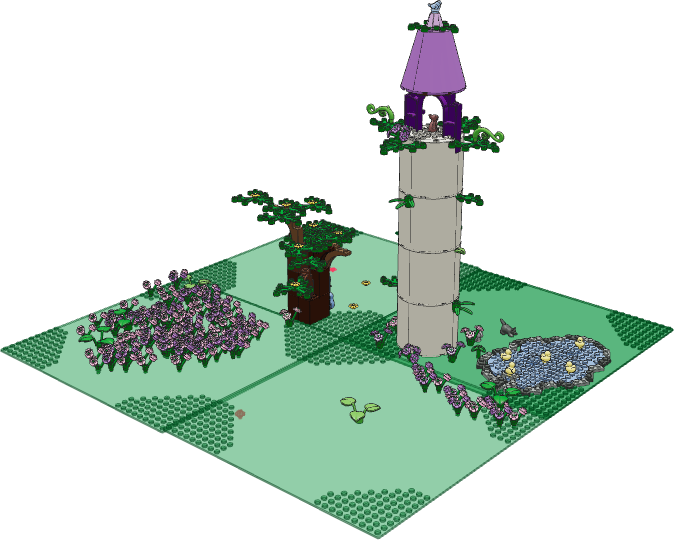
\includegraphics[width=\textwidth]{./figures/rapunzel.png}
        \caption{Rapunzel tower}
        \label{fig:rapunzel}
    \end{subfigure}
    \caption{LEGO product designs proposed by the teams during the workshop.}
    \label{fig:kinderuni}
\end{figure}

For all teams, one requirement was that they uploaded the current state of their digital LEGO designs every hour to CADdrive, so that the design process can be reconstructed and visualized.
For teams including two members, another challenge was dividing their work into two independent modules, developing the two modules separately, and integrating the modules at the end of the workshop day.
Three out of nine two-member teams managed to master this challenge (as, e.g., shown in Figure~\ref{fig:school-sub}), while three two-member teams decided not to divide their work, but decided to work together in front of one computer only.
The remaining three two-member teams failed integrating their work.

\begin{figure}[htbp]
    \centering
    \begin{subfigure}[b]{0.2\textwidth}
        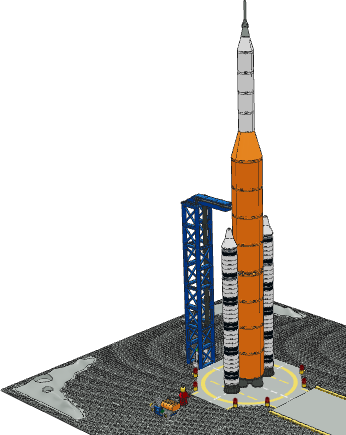
\includegraphics[width=\textwidth]{./figures/space_rocket.png}
        \caption{Rocket component}
    \end{subfigure}
    \hspace{0.05\textwidth}
    \begin{subfigure}[b]{0.6\textwidth}
        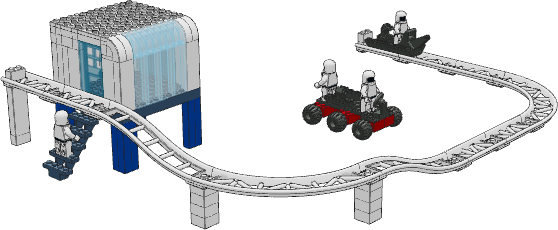
\includegraphics[width=\textwidth]{./figures/space_station.png}
        \caption{Station component}
    \end{subfigure}
    \caption{Independent components of the space station LEGO product idea.}
    \label{fig:school-sub}
\end{figure}

\section{Evaluation results}
\label{sec:discussion}

After conducting the experiments from the previous section, we performed a systematic evaluation on the Master-level courses as well as an informal feedback round on the workshop to understand the current quality of our educational offering in these different contexts.
For systematic evaluation, we developed a questionnaire assessing the prior experience of the course participants in different knowledge domains as well as the learning experience during the course.
In the following, we first present the results of the assessment of prior expierience in Section~\ref{sec:prior} before going into the details of the assessment of the learning experience in Section~\ref{sec:learning}.

\subsection{Prior experience}
\label{sec:prior}

Figure~\ref{fig:before} summarizes the results of the assessment of prior experiences of our Master-level course participants.
In our questionnaire we assessed prior experiences in different fields such as CAD/CAM (\textit{medium}), simulation (i.e.\ FEM/CFD/MBS/MPS/DES; \textit{low}), PDM/PLM (\textit{high}), QFD/DSM (\textit{low}), product management/design (\textit{medium}), systems/requirements/mechanical/electrical/software engineering (\textit{high}), as well as project management, agile methodology, and design thinking (\textit{high}).
Note that in each category the participants selected between novice, junior, professional, senior, and expert experience levels, which we aggregated to low, medium, and high levels here for gaining a bigger picture.

\begin{figure}[htbp]
    \centering
    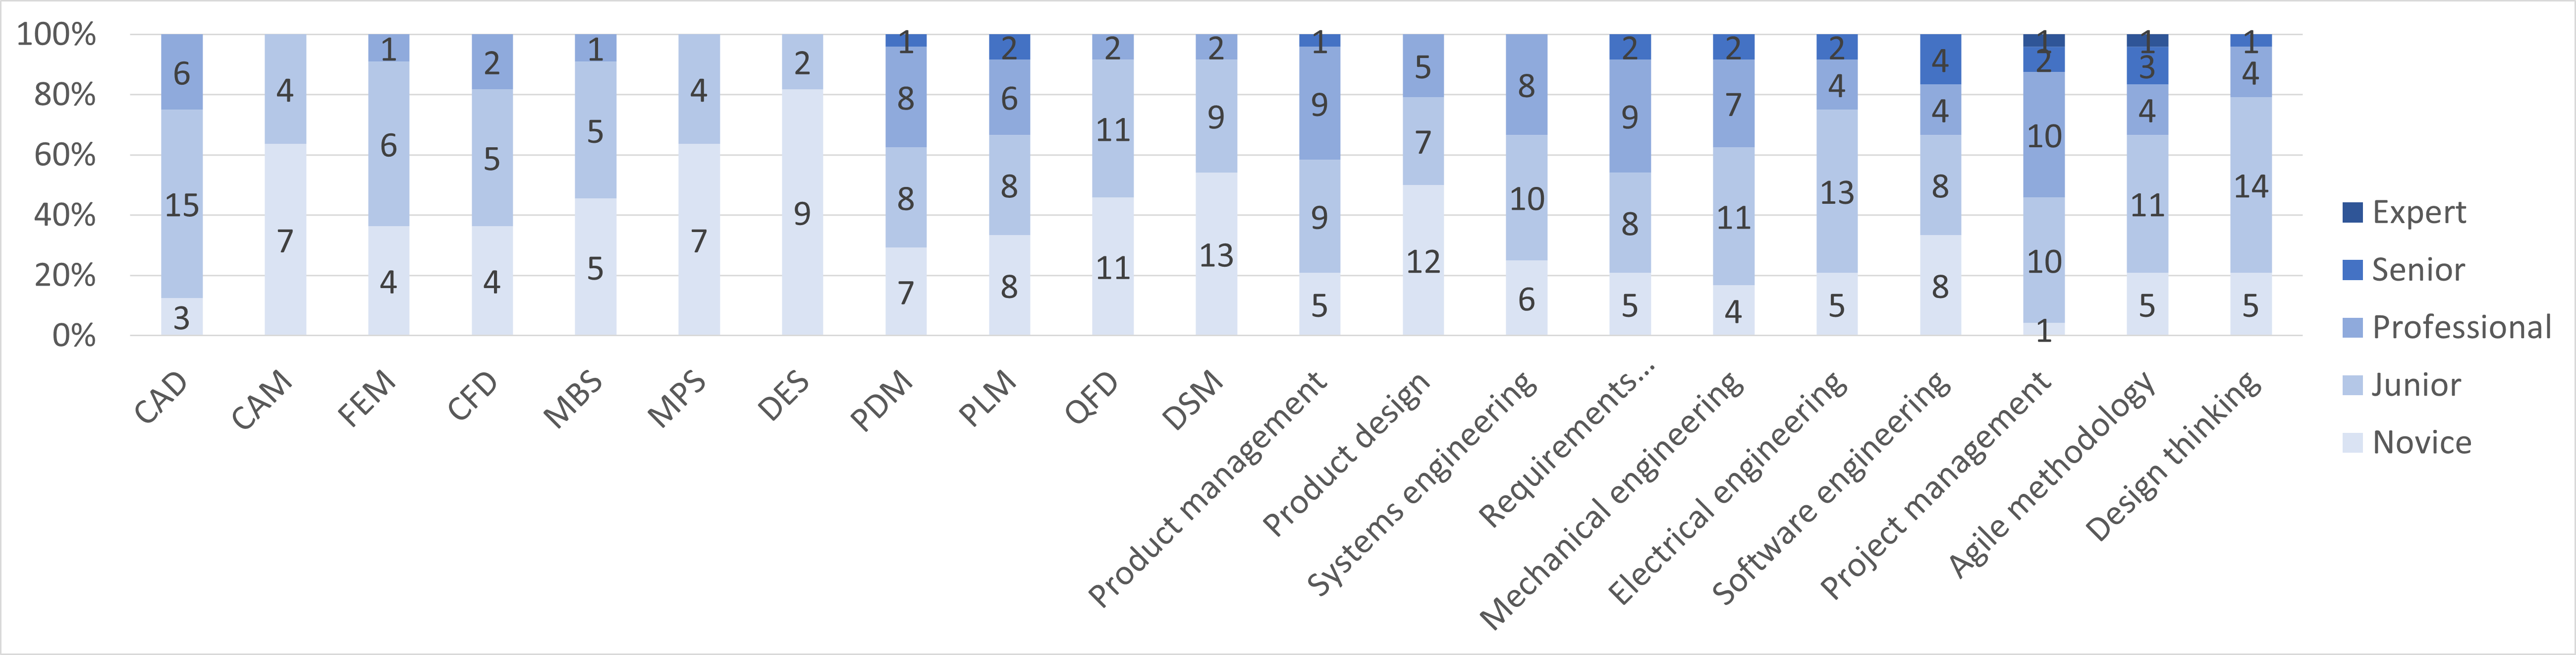
\includegraphics[width=\textwidth]{./diagrams/before.png}
    \caption{Summary of prior experience in different knowledge areas.}
    \label{fig:before}
\end{figure}

\subsection{Learning experience}
\label{sec:learning}

For assessing the learning experience during the two Master-level courses on product design and systems engineering, the questionnaire included a quantitative and a qualitative section.
In the quantitative section we assessed the general learning experience, the learning experience in different knowledge areas (e.g.\ digital collaboration and agile methodology), and the learning experience with the different software tools (e.g.\ CADdrive and LeoCAD) as described in Section~\ref{sec:quantitative}.
In the qualitative section we asked the participants about ideas for improvement of the two different course concepts as well as the software tools employed as described in Section~\ref{sec:qualitative}.

\subsubsection{Quantitative feedback}
\label{sec:quantitative}

TODO

\begin{figure}[htbp]
    \centering
    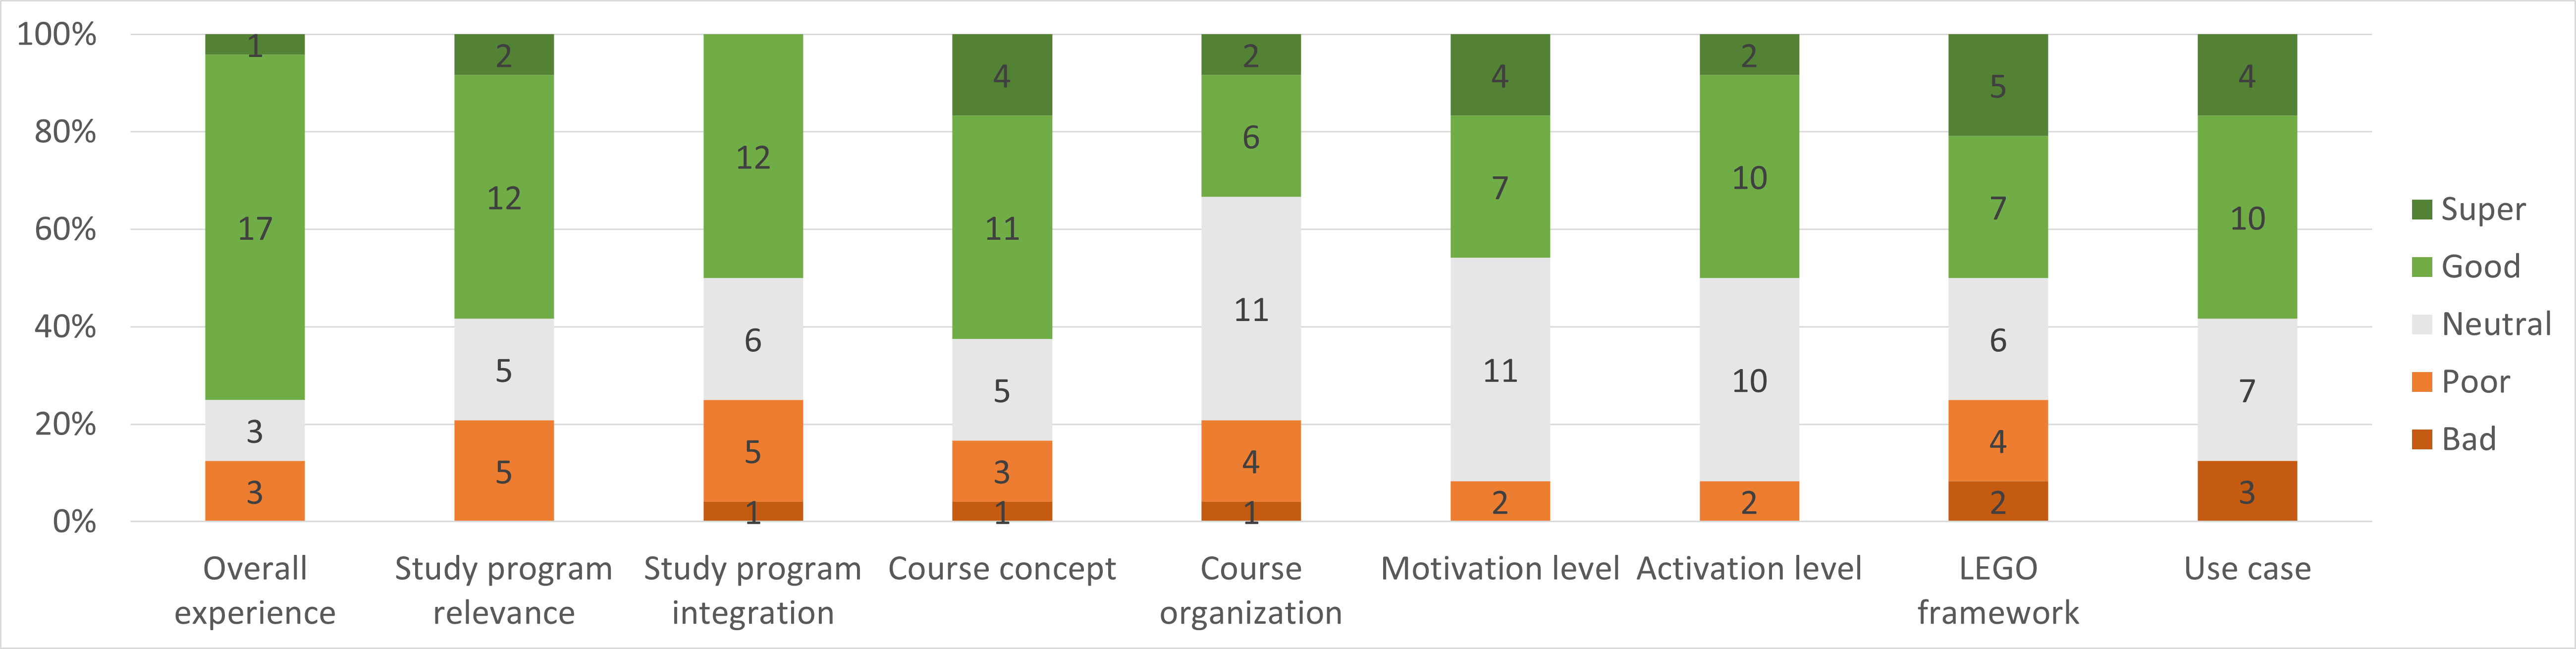
\includegraphics[width=\textwidth]{./diagrams/after-general.png}
    \caption{Summary of general learning experience during the course.}
    \label{fig:after-general}
\end{figure}

TODO

\begin{figure}[htbp]
    \centering
    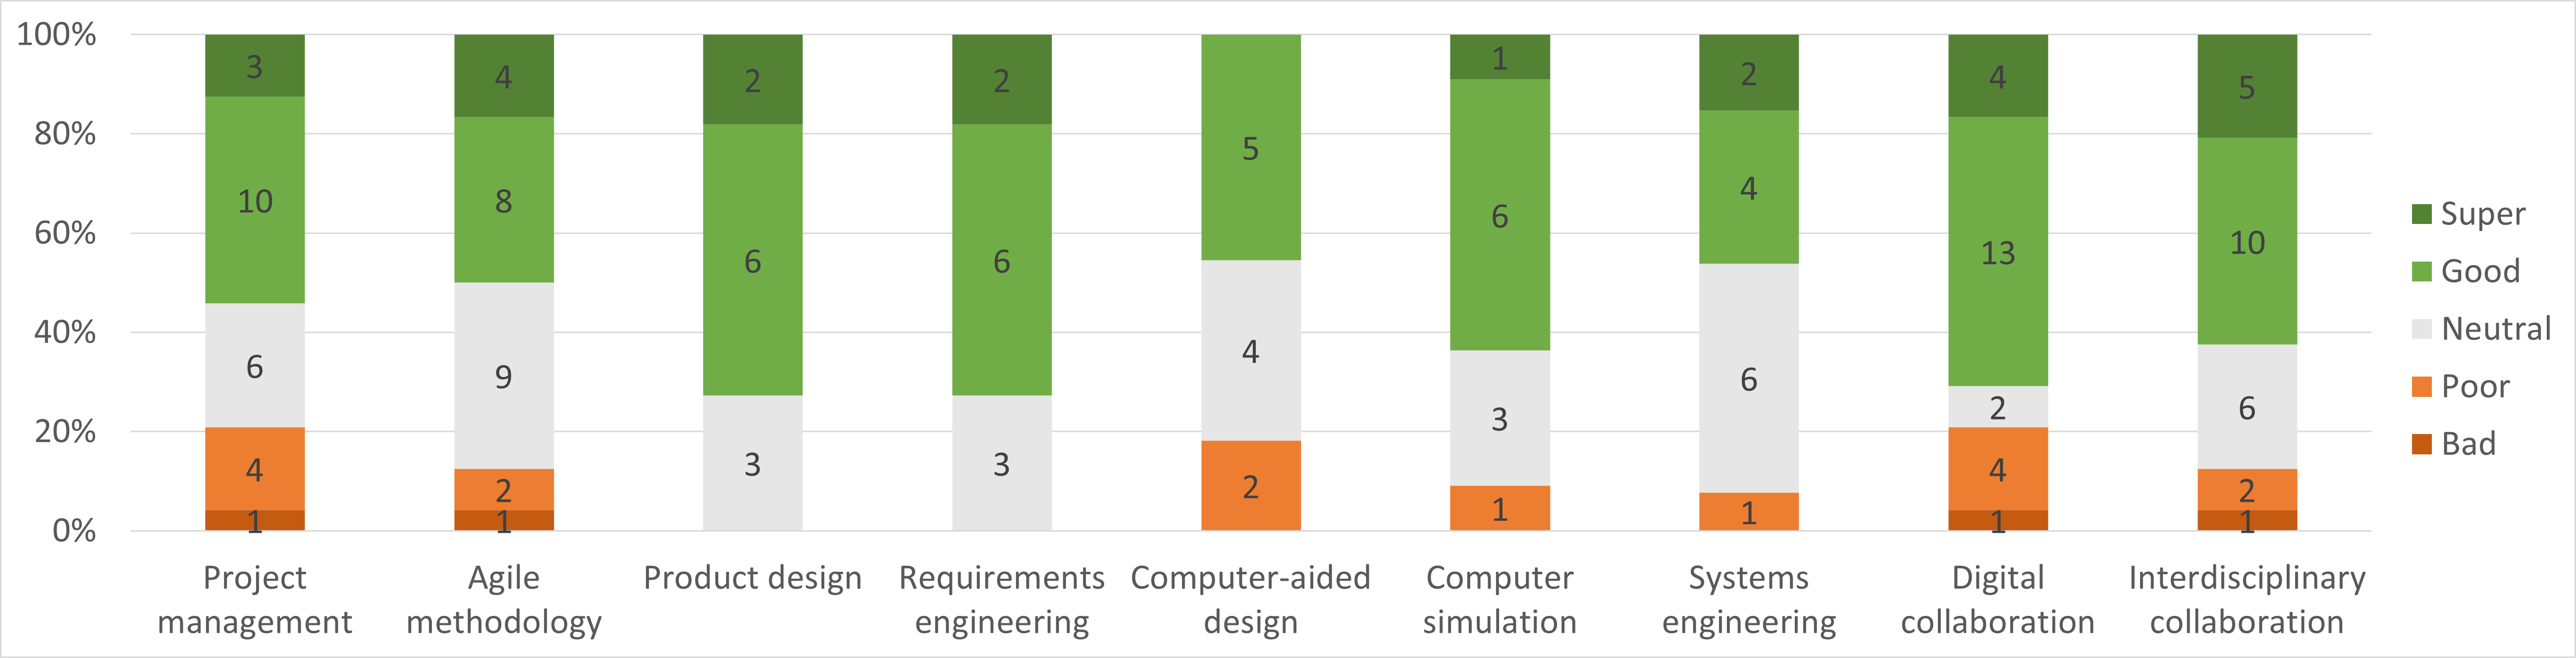
\includegraphics[width=\textwidth]{./diagrams/after-knowledge.png}
    \caption{Summary of learning experience in different knowledge areas.}
    \label{fig:after-knowledge}
\end{figure}

TODO

\begin{figure}[htbp]
    \centering
    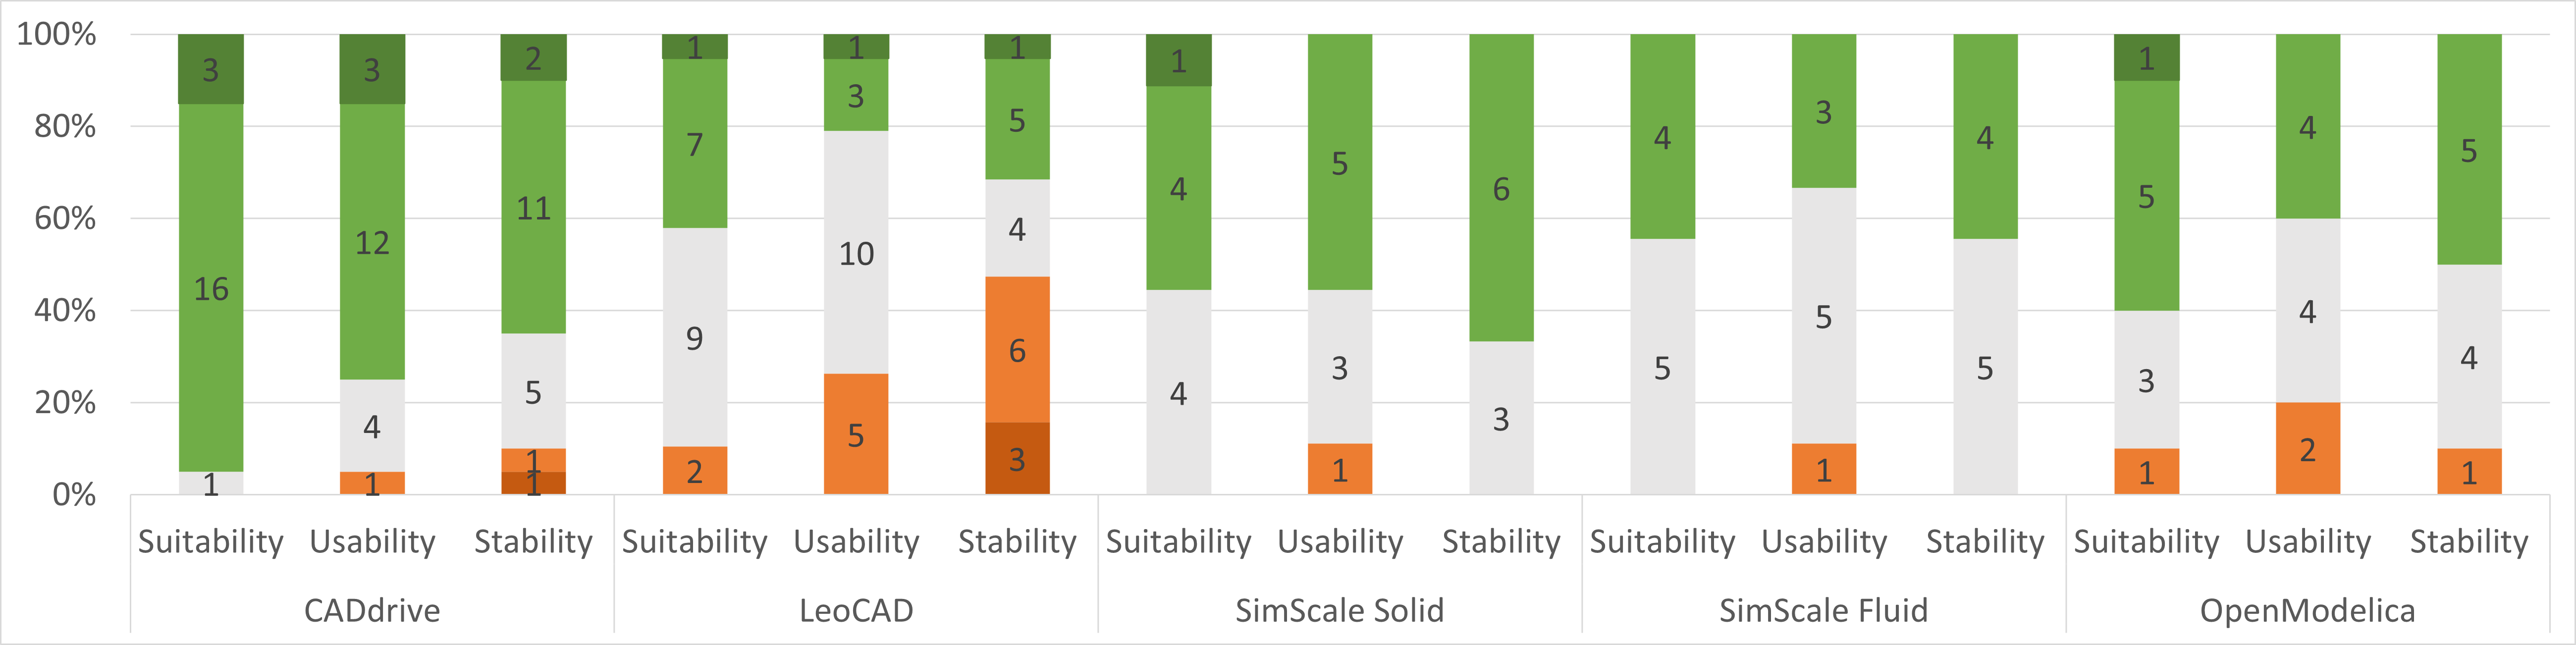
\includegraphics[width=\textwidth]{./diagrams/after-software.png}
    \caption{Summary of learning experience with the different software tools.}
    \label{fig:after-software}
\end{figure}

\subsubsection{Qualitative feedback}
\label{sec:qualitative}

TODO

\section{Conclusions}
\label{sec:conclusion}

TODO

\paragraph{Summary}

TODO

\paragraph{Outlook}

TODO

\begin{Backmatter}

\bibliography{main}
\bibliographystyle{plainnat}

\end{Backmatter}

\end{document}